\section{Introduction}
\section{Tools}
\subsection{IDE}
Visual Studio Code was used for this project due to prior experience with the IDE. It is also one of the most popular tools in the industry 
as shown by the Stack Overflow Developer Survey\cite{StackOverflowDeveloper} and the TOP IDE Index\cite{TOPIDETop}.
VS Code has excellent support for many programming languages, and with a wealth of community made extensions there are many tools to aid with development.
\subsection{Version Control}
Version control is a system that records changes to a file or set of files over time so that you can recall specific versions later.\cite{GitVersionControl}
Using version control with an external hosting provider also makes working over several computers easy which will be useful for this project, and it ensures everything is backed up remotely.
Git was chosen for version control as it is the industry standard, with GitHub being used as the hosting provider.
\subsection{Database Visualisation}
Neo4j has two tools for database visualisation as part of the AuraDB web interface; Bloom and Browser. Bloom is used to 
visualise the data in a graph as has been discussed in the design chapter previously. Browser is used to test CYPHER queries on the database.
CYPHER is the query language created by Neo4j for retrieving data from their graph databases. As shown Figure 4.1, the user can enter a 
query and have the data returned as a graph, table (represented as a series of JSON objects), raw text and as code (JSON objects).
This is useful for quickly testing CYPHER queries and debugging database interactions.
\begin{figure}[h]
    \centering
    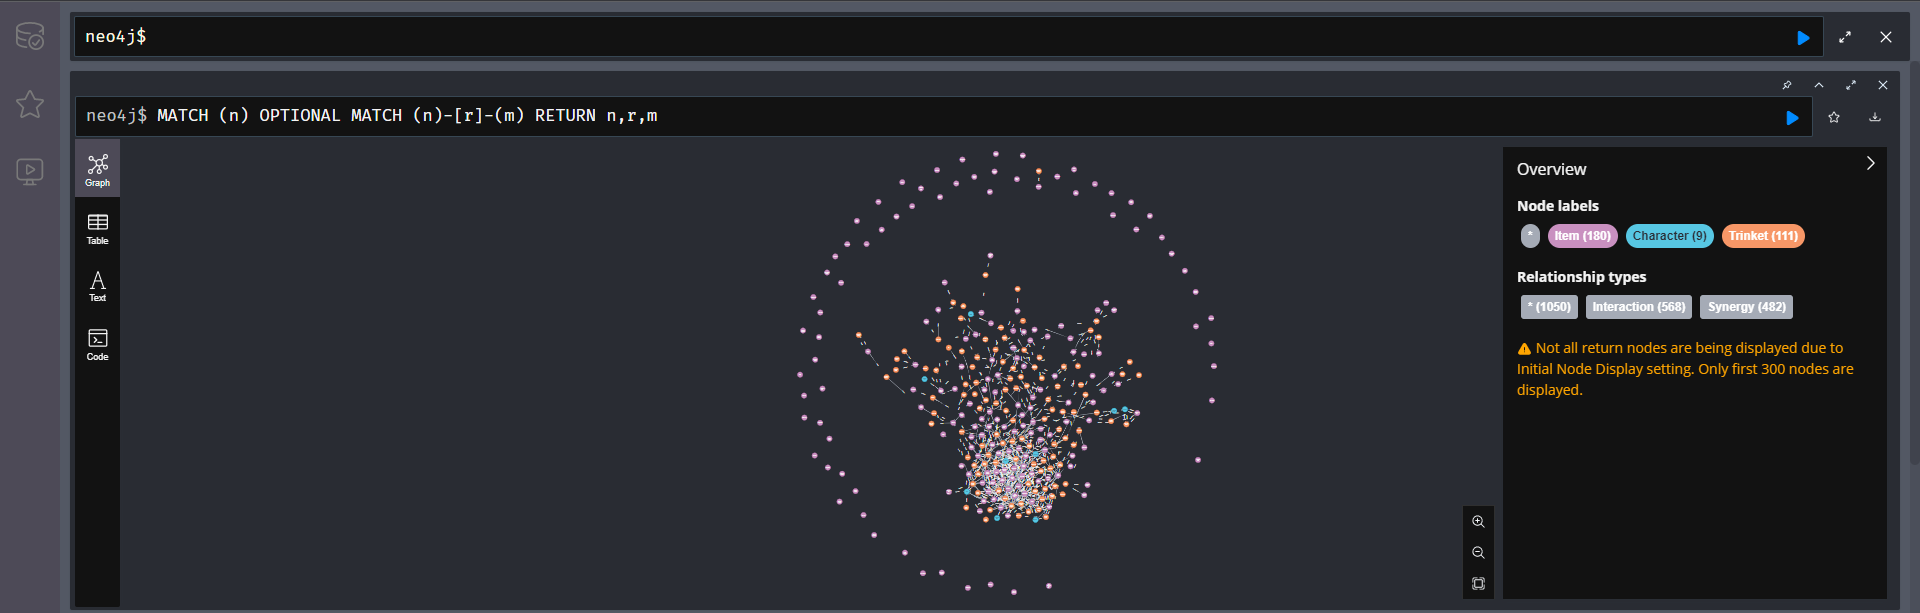
\includegraphics[width=0.8\textwidth]{neo4jBrowser}
    \caption{AuraDB Browser}
\end{figure}
\section{Libraries}
\subsection{Data Processing}
\begin{description}
    \item[Beautiful Soup] - A Python library for pulling data out of HTML and XML files\cite{BeautifulSoupDocumentation}. 
    Used to parse the XML dump and extract data for the database.
\end{description}
\subsection{Client Side}
\begin{description}
    \item[Cytoscape] - A JavaScript library that `allows you to easily display and manipulate rich, interactive graphs'\cite{franzCytoscapeJsGraph2016}. 
    Used in this project to display the data in graphs to the user.
    \item[Material] - An Angular specific library containing material design components, used in this project to quickly create UI components.
\end{description}
\subsection{Server Side}
\begin{description}
    \item[Neomodel] - An Object Graph Mapper (OGM) for the Neo4j graph database\cite{NeomodelDocumentationNeomodel}, used to define Django models for access database data.
    \item[django-cors-headers] - A Django App that adds Cross-Origin Resource Sharing (CORS) headers to responses. This allows in-browser requests to your Django application from other origins.\cite{yiuDjangocorsheadersDjangocorsheadersDjango} 
    this is required for the front end and back end to communicate properly.
\end{description}
\section{Data Processing}
The first major section of the implementation was setting up the graph database and getting the data required to do so.
\subsection{Finding Data Source}
The initial project brief suggested using the Fandom wiki for the data source as Fandom wikis have the option for downloading 
an XML dump from the \verb|Special:Statistics| page. As discussed in section 2.3, the Fandom wiki is also the most comprehensive 
source of data about the game, especially regarding the item interactions. The XML dumps are not always kept up to date, so while 
a new dump was being requested other options for the data source were investigated. This included investigating the game files, where 
all the resource files have been packed in to \verb|A| files. In the folder containing the resource files there is a readme which explains 
that this was done to prevent spoilers and any secrets being found through the files. A resource extractor tool is included with later versions of the game, 
however the files do not contain any information regarding the interactions of items.\par
Once received, the updated XML dump presented its own challenges, the first being its size, at just under 500,000 lines long and around 20MB it was too 
large for most text editors to load with syntax highlighting. This made it difficult to understand the structure of the data as the XML tags became harder 
to pick out from regular text. Aside from a small preamble, all the data in the file is contained in a series of \verb|page| elements, which unsurprisingly represents a page on the site.
Each page element has a similar structure to the below example (Fig. 4.2).
\begin{figure}[H]
    \begin{lstlisting}[language=XML]
        <page>
        <title>Template:</title>
        <ns>10</ns>
        <id>161</id>
        <redirect title="Template:*" />
        <revision>
          <id>161</id>
          <timestamp>2014-09-16T20:27:12Z</timestamp>
          <contributor>
            <username>Maintenance script-gpuser</username>
            <id>41555837</id>
          </contributor>
          <comment>&amp;lt;default import&amp;gt;</comment>
          <origin>161</origin>
          <model>wikitext</model>
          <format>text/x-wiki</format>
          <text bytes="24" sha1="2dwqfi7oey6311xkwxu3dhjasn8gfsi" xml:space="preserve">#redirect [[Template:*]]</text>
          <sha1>2dwqfi7oey6311xkwxu3dhjasn8gfsi</sha1>
        </revision>
      </page>
    \end{lstlisting}
    \caption{Example page format}
\end{figure}

The important parts to note from this is that the \verb|title| element is the web page title and the \verb|text| element contains the data to be displayed (or in this case a redirect to another page).
There doesn't appear to be a particular order to the pages and due to the formatting of the file it can be hard to tell where one page ends and another begins.
\subsection{Data Extraction}
Due to the structure of the XML data, the easiest way to extract the data is to use the title tags for each page to find the relevant and pages 
and then pull the data from the text tag. The XML file contains collections pages which each contain a list of items available in each version of the game, this can be 
used to get a list of all the item names. Character names are fetched from the \verb|Characters| page. This has a list of links to the character pages, from which the names can be extracted using RegEx. 
Unfortunately, the same does not exist for trinkets as the page that would contain that list instead uses a template which autofills the data. 
As a temporary fix, the list of trinkets is fetched from a hardcoded file.
\begin{figure}[H]
    \begin{lstlisting}[language=Python]
        ITEM_REGEX = re.compile("content =(.*?)}}", flags=re.DOTALL)

        def _get_item_names(self):
            collection = self.soup.find("title", text="Collection Page (Repentance)").find_parent("page").find("text").text
            return [
                x.strip()
                for x in ITEM_REGEX.search(collection)[1].replace("\n", "").replace("Number Two", "No. 2").split(",")
            ]
    \end{lstlisting}
    \caption{Function that returns the list of item names}
\end{figure}

Figure 4.3 shows the code used for getting the list of item names, similar code has been used for getting character names.
\verb|re| is a Python library that provides regular expression matching operations. In the data extraction script a series of 
compiled RegEx statements are defined as constants, \verb|ITEM_REGEX| being one of them. These are used through the script 
to pull data from the XML file based on the format of the data. Here BeautifulSoup is used to find the title tag that contains the text 
`Collection Page (Repentance)', this is then used to get its parent and to search that for the text element. 
To get the data from the string of text the RegEx statement is used to search for a string that starts with \verb|content =| and ends with \verb|}}|.
The \verb|(.*?)| matches a string of any characters of any length non-greedily and puts it in a match group. 
This means it will match against any character until the first instance of \verb|}}| and the object returned is subsriptable to get the match groups.
Accessing group 0 is the whole match which will included the \verb|content =| and \verb|}}|, accessing group 1 is the first (and in this case only) match group.
The string returned by accessing the match group then has new line characters removed and and is split into a list using the commas.
Each value in this array then has any leading and trailing whitespace removed using \verb|strip()| and a listcomprehension.
There is an extra step needed here due to the nature of the XML data and that is manually replacing the item name for `Number Two'.
This had to be done as the name appears in several different formats throughout the data, but the only one that has a page with data in is `No. 2'. 
The rest of the pages just redirect back to that page and so instead of handling the redirect it is easier to catch and replace the different formats when they appear.

got list of names now what?
- iterate over list of all title tags and use if statements to check if its one we care about
- faster to do that then search for each name we do care about because accessing all the data in BeautifulSoup takes a while(?)
- in each loop it: checks its a tag we care about > gets text and id > check if ID is none > extract and append data to array > add id to lookup > add synergies/interactions to list
- once we have the data for all the nodes we can work on the relationships
- using the lists created before each entry is processed by using regex to get any tags and then looking up their id to find a target ID
- source id, target id and descripton is then put into new array
- theres a bunch of stupid data that has be caught using if statements and corrected
\subsection{Cleaning the Data}
regex is used again to clean the sections of text
The text contains lots of tags for vairous features in the wiki such as dlc tags and links to other pages
turns bullet pointed lists into nested arrays
\subsection{Importing into Database}
neo4j has a data importer tool which uses csv files to populate a data model
csv files were generated from the data objects in python
\begin{figure}[H]
    \centering
    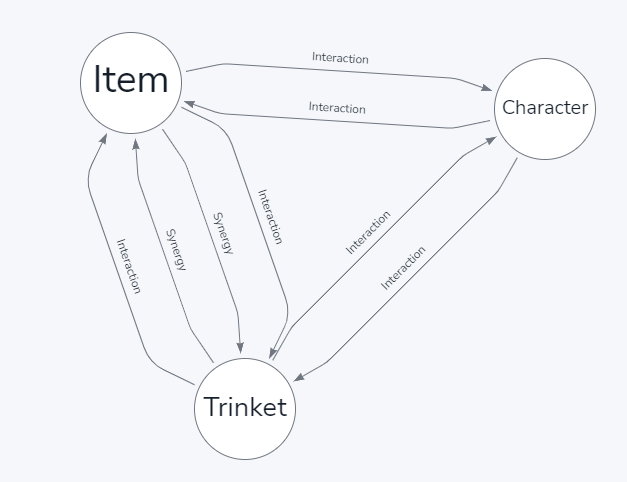
\includegraphics[scale=0.4]{dataImport}
    \caption{Database Model in Neo4j Data Importer}
\end{figure}
\todo{Database model is wrong}
\section{Web Stack}
creating django project with an api app and a main "query" app
api app contains webserver (?) and the settings
each app then contains the the models, views and urls etc
urls.py defines what functions get called by each urls
views.py defines the functions used by urls, these functions contain all the functionality the user interacts with,
each function takes in a request from the url and depending on the type of request (e.g get, post etc), performs the relevant action
models.py contains classes each of which represent a type if data entity

create a angular project and any components
(explain angular project structure)
each component represents a "screen"
(explain component structure)

There is a shared services file, this defines the interaction with the backend api
the address of the backend server is defined in there and the functions that make the http requests

each project has it's own git repo which are then submoduled into the main project repo
\section{Database Interaction}
Used neomodel to define classes for each entity and relationship type, these classes contain methods for retrieving data
Getting all nodes is very easy due to built in methods, however these do not exist for relationships
so to get all relationships you have to perform a cypher query to get them
\section{Client Side}
first made tables to check everything worked
found that the json like object created by neomodel couldn't be interpreted by the front, so had to manually make a get method for each class
This causes getting large amounts of data (relationships) to take quite a long time

I created a second component to show the data in a graph form as per my initial design
To do this I used cytoscape.js (more info)
had to rewrite how the data is formatted when sent to the front end so that it matchs what cytoscape expects
still takes a long time to get data from backend 
so decided to write it to a json file so at least for quicker debugging it can load directly from the file
tweaked some settings to make the graph easier to read

\section{Conclusion}